\documentclass[a4paper,twoside]{article}

\usepackage{epsfig}
\usepackage{subfigure}
\usepackage{calc}
\usepackage{amssymb}
\usepackage{amstext}
\usepackage{amsmath}
\usepackage{amsthm}
\usepackage{multicol}
\usepackage{eurosym}
\usepackage{apalike}
\usepackage{epstopdf}
\usepackage{SCITEPRESS}     % Please add other packages that you may need BEFORE the SCITEPRESS.sty package.
\usepackage[utf8]{inputenc} %Codificacion utf-8

\subfigtopskip=0pt
\subfigcapskip=0pt
\subfigbottomskip=0pt

\begin{document}

\title{Adaptative and personalized web framework for searching data using flexible queries  \subtitle{} }

\author{\authorname{Victor Pablos Ceruelo\sup{1}, Dan Seeruttun - - Marie\sup{1} and Susana Muñoz Hernandez\sup{2}}
\affiliation{\sup{1}PHD in ...,  Universidad Politecnica de Madrid, My Street, MyTown, MyCountry}
\affiliation{\sup{2}Student in Software Engineering, Universidad Politecnica de Madrid, Rennes, France}
\affiliation{\sup{3}Computer Science...,  Universidad Politecnica de Madrid, MySecondTown, MyCountry}
\email{\{victorpablosceruelos, dan.seeruttun\}@gmail.com, susana@fi.upm.es}
}

\keywords{Active learning, Fuzzy logic, Database}

\abstract{The abstract should summarize the contents of the paper and should contain at least 70 and at most 200 words. The text must be set to 9-point font size.}

\onecolumn \maketitle \normalsize \vfill

\section{\uppercase{Introduction}}
\label{sec:introduction}

\noindent When trying to model a problem, assigning each concept to a term and an universal meaning is very important. These names must be very clear for anyone. However, problems can appear during the modelization of a fuzzy or subjective problem, where terms meaning vary and are not clear. 

\noindent For instance, trying to model the concept of the predicate expensive car is difficult because it involves each person own idea of expensive to represent it.  Secondly, how can a car be defined with an expensive and non expensive term ? If sticking to the reality is an objective, being able to define the expensiveness of any product is the key.

\noindent Thus a better representation of the predicate is needed, associating a cost and its match with the predicate is the idea. That's introducing the concept of truth value, seen in (Citation Victor Thesis), a value that will represent the match between fuzzy values and their predicates, or in our example costs and the predicate expensive. With this modelization, it will become possible to search through databases, coupling truth values and fuzzy predicates and even going further by personalizing predicate to users.
In this paper, FLESE will be presented, an implementation of the fuzzy concept through databases, adaptative and able to personalize to each user.

%\section{\uppercase{RFUZZY}}

\section{\uppercase{FLESE}}

\section{\uppercase{ADAPTATIVE PERSONALIZED FRAMEWORK}}

\subsection{USER PERSONALIZATION}

\noindent Flese application brings the treatment of the fuzzy queries but it does not solve the problem of the subjectiveness of the fuzzy queries. Indeed, an expensive car does not have the same meaning for everyone.\\

\noindent The point of the user personalization is to give to the user the opportunity to modify the definition of the fuzzy predicates, thus to overcome the subjectivity of the vocabulary used. Moreover, a personalization does not affect other users, so each user can create his own definitions of the same predicate to access the same database using Flese. The database file will then contain all users personalization.\\

\noindent For instance, if the user is looking for an expensive car, he will find the following solutions: \\

\begin{table}[h]
\caption{Results of simple expensive car query}\label{tab:simpleQuery1} \centering
\begin{tabular}{|c|c|c|c|}
  \hline
  N0 & Name & Price & Truth value\\
  \hline
  1 & VW Caddy & 45000 & 1\\
  \hline
  2 & Alfa Romeo & 30000 & 1 \\
  \hline
  3 & Aston Martin & 150000 & 1 \\
  \hline
  4 & Ford S Maxi & 30000 & 1 \\
  \hline
  5 & Audi TT & 40000 & 1 \\
  \hline
  6 & Audi Quattro & 48000 & 1 \\ 
  \hline
\end{tabular}
\end{table}

\noindent The 6 first results will be expensive car with a truth value of 1, this table of results will not please a rich user, that will be interested in a higher cost for the predicate expensive. \\

\noindent Then he will assign a truth value to different ranges of prices, from inferior to 10000 \euro to more than 1000000 \euro. A rich user may personalize this predicate imposing that a car valued at 30000 \euro is not really expensive (truth value = 0.40) and a car valued at 1000000 \euro is very expensive (truth value = 1). After being modified, a message appears confirming the modification. \\

\begin{figure}[!h]
  %\vspace{-0.2cm}
  \centering
   {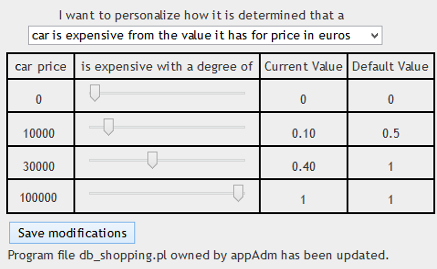
\epsfig{file = pers.png, width = 8cm}}
  \caption{This caption has one line so it is centered.}
  \label{fig:example1}
 \end{figure}

\noindent After having modified the predicate, the user can still have a look to the default value of the predicate in case of he is lost. This part remains important to help the user to get back from a wrong personalization. The result of the query is the following:  \\ 

\begin{table}[h]
\caption{Results of fuzzy expensive car query}\label{tab:solveQuery1} \centering
\begin{tabular}{|c|c|c|c|}
  \hline
  N0 & Name & Price & Truth value\\
  \hline
  1 & Aston Martin & 150000 & 0.47 \\
  \hline
  2 & VW Caddy & 45000 & 0.41\\
  \hline
  3 & Audi TT & 40000 & 0.41 \\
  \hline
  4 & Audi Quattro & 48000 & 0.41 \\ 
  \hline
  5 & Alfa Romeo & 30000 & 0.4 \\
  \hline
  6 & Ford S Maxi & 30000 & 0.4 \\
  \hline
\end{tabular}
\end{table}

\noindent Asking for his expensive car, the user knows by reading the truth values that there is no expensive car according to his definition. The more expensive car has a truth value of 0.47. However, he can still compare the price of the other cars,
The owner of the file can decide which predicate he wants to authorize the personalization. He keeps the control on the file, he can impose a default value of the fuzzification before any personalization. \\

\subsection{MACHINE LEARNING FOR IMPROVING SEARCHING CRITERIA}

\noindent Starting considering an increasing number of users, it becomes interesting to search for better predicate criteria. Indeed, the users joining the application after the others can benefit from the others data. Knowing that people share some predicate personalization can lead to an improvement of the criteria for the newcomers. In that sense, Flese changes the values of the default function for the newcomers' and non personalized's predicate according to what is most representative to the users. \\

\noindent Theses changes will have no effect on the parametrized fuzzification if it has been already changed. For example, for the expensive predicate, if we introduce more rich people than poor, the definition of the predicate will adapt to the situation, following the rich people predicates. \\

\noindent The searching criteria will then adapt to the population of the users. Even after deciding to invert the population rate, by adding more poor people, the predicate criteria will be personalized by the new population to fit their idea. In that case, the criteria will represent more the poor people.
For instance, if most of the people consider that 10000 \euro and 30000 \euro is not expensive, the default expensive predicate will adapt according to it. Here is an example showing it:


\section{\uppercase{Copyright Form}}

\noindent For the mutual benefit and protection of Authors and
Publishers, it is necessary that Authors provide formal written
Consent to Publish and Transfer of Copyright before publication of
the Book. The signed Consent ensures that the publisher has the
Author's authorization to publish the Contribution.

The copyright form is located on the authors' reserved area.

The form should be completed and signed by one author on
behalf of all the other authors.

\section{\uppercase{Conclusions}}
\label{sec:conclusion}

\noindent Please note that ONLY the files required to compile your paper should be submitted. Previous versions or examples MUST be removed from the compilation directory before submission.

We hope you find the information in this template useful in the preparation of your submission.

\section*{\uppercase{Acknowledgements}}

\noindent If any, should be placed before the references section
without numbering. To do so please use the following command:
\textit{$\backslash$section*\{ACKNOWLEDGEMENTS\}}


\vfill
\bibliographystyle{apalike}
{\small
\bibliography{example}}


\section*{\uppercase{Appendix}}

\noindent If any, the appendix should appear directly after the
references without numbering, and not on a new page. To do so please use the following command:
\textit{$\backslash$section*\{APPENDIX\}}

\vfill
\end{document}

